\chapter{Wavelets}
De Fouriertransformatie bestaat al honderden jaren en is een grote speler geworden in de \emph{signal processing}. Een groot nadeel van deze transformatie is dat zij slecht reageert op discontinue signalen door de globale dragers van de basisfuncties. Hierdoor worden alle Fourierco\"effici\"enten be\"invloed door een discontinu\"iteit.

In de loop van de vorige eeuw is een nieuwe transformatie ontstaan met een eigenschap die de Fouriertransformatie nooit kende. Deze noemt men nu ook wel de Wavelettransformatie.

\begin{definitie}
  Een wavelet is simpelweg een functie $\psi: \R \to \R$ die voldoet aan
  \[
  \int_{-\infty}^{\infty} \psi(t) dt = 0.
  \]
  Met deze functie $\psi$ kunnen we een familie functies $\psi_{u,s}$ bouwen door middel van schaling en translatie:
  \[
  \psi_{u,s}(t) := \frac{1}{\sqrt{s}} \psi\left(\frac{t-u}{s}\right).
  \]
\end{definitie}

Deze familie geeft aanleiding tot een Wavelettransformatie $W_f$ van $f$:
\[
W_f(u,s) = \int_{-\infty}^\infty f(t) \psi^*_{u,s}(t) dt.
\]

Het is nu mogelijk om wavelets te construeren die met deze schaling en translatie een basis voor de $L_2(\R)$ vormen. Over het algemeen kijken we dan naar
\[
\left\{ \psi_{j,n}(t) = \sqrt{2^j} \psi\left( 2^j t - n\right) : (j,n) \in \Z^2 \right\}.
\]
De kunst is nu om de basiselementen loodrecht op elkaar te laten staan, zodat er een orthogonale (en dus een orthonormale) basis gevormd wordt.

Figuurtje van voorbeeld TODODOO.

\begin{gevolg}We kunnen een functie $f$ in $L^2(\R)$ schrijven in deze basis:
  \[
  f(t) = \sum_{j=-\infty}^{\infty} \sum_{n=-\infty}^{\infty} \langle f, \psi_{j,n} \rangle \psi_{j,n}(t),
  \]
  waarbij $\langle \cdot, \cdot \rangle$ het standaardinproduct op de $L_2(\R)$ aangeeft.
\end{gevolg}

Het grote nadeel van de Fouriertransformatie maakt compressie van discrete signalen moeilijk. Veel van deze wavelets worden nu z\'o geconstrueerd dat dit probleem (deels) verholpen wordt. We zijn namelijk op zoek naar een wavelet die een eindige drager heeft. Het blijkt dat deze bestaat en dat er zelfs een hele grote verzameling wavelets is, elk met eigen gewilde eigenschappen.

Omdat wij naar de toepassing van wavelets binnen de beeldcompressie bekijken, zijn we natuurlijk vooral ge\"interesseerd in het discrete geval. We kijken dus naar de benadering van $f$. Dit geeft aanleiding tot een rij geneste ruimtes die uiteindelijk naar de $L_2(\R)$ toe gaat:

\begin{equation}
  \label{multires}
  V_0 \subset V_1 \subset \ldots \subset L_2(\R)
\end{equation}
genaamd een multiresolutie.
\begin{definitie}
  Een rij geneste ruimtes $\{ V_j: j \in \N_0 \}$ zoals in~\ref{multires} heet een multiresolutie wanneer voldaan wordt aan de volgende eigenschappen:
  \begin{eqnarray}
    \forall j, k: f(t) \in V_j \implies f(t - 2^j k) \in V_j, \\
    \forall j: V_{j-1} \subset V_j, \\
    \forall j: f(t) \in V_j \iff f(t/2) \in V_{j-1}, \\
    \bigcup_{j=0}^{\infty} V_j = \lim_{j\to\infty} V_j = L_2(\R), \\
    \text{ Er is $\phi: \R \to \R$ zo dat $\{ \phi(t-n): n \in \Z \}$ een orthonormale basis voor $V_0$ is.}
  \end{eqnarray}
\end{definitie}

\begin{voorbeeld} We bekijken een multiresolutie van stuksgewijs constante functies. De ruimte $V_j$ wordt hiermee
  \[
  V_j = \left\{ g(t) \in L_2(\R): g(t)\text{ is constant voor }t \in [n 2^{-j}, (n+1)2^{-j}) \right \}
    \]
    met $n \in \Z$. De basisfunctie $\phi$ voor $V_0$ wordt in dit geval $\phi(t) = 1_{[0,1)}(t)$.
\end{voorbeeld}

\section{Schalingsfuncties}
Gegeven zo'n orthonormale basis voor $V_0$ willen we graag een orthonormale basis voor $V_j$ construeren.
\begin{stelling}[{\cite[T7.1]{mallat}}]
  Laat $\{ V_j \}$ een multiresolutie en laat $\{\phi(t-n) \}$ de basis voor $V_0$. Laat verder
  \[
  \phi_{j,n}(t) := \sqrt{2^j} \phi\left( t2^j - n \right).
  \]
  Dan is $\{ \phi_{j,n}: n \in \Z \}$ een orthonormale basis voor $V_j$. De functie $\phi$ is ook wel de \emph{schalingsfunctie}.
\end{stelling}
\subsection{Benadering} De orthogonale projectie van $f$ op $V_j$ is, zoals we weten, de beste benadering van $f$ in $V_j$. Deze is nu te vinden door
\[
P_{V_j} f = \sum_{n=-\infty}^\infty \langle f, \phi_{j,n} \rangle \phi_{j,n}.
\]
De co\"effici\"enten $a_j[n] = \langle f, \phi_{j,n} \rangle$ geven ons op deze manier een discrete benadering van $f$ op resolutie $2^j$.

\section{Filters}
Wanneer we een schalingsfunctie $\phi$ defini\"eren (en dus een $V_0$), dan lijkt $V_1$ (en dus $V_j$) al redelijk beschreven te worden.\footnote{In stelling \ref{filter} wordt bewezen dat deze hele multiresolutie vast ligt.} We zullen daarom deze schalingsfunctie nader onderzoeken.

Per definitie van de multiresolutie weten we dat $V_{j-1} \subset V_j$. In het bijzonder geldt dat $\phi(t) \in V_0 \subset V_1$ en omdat $\{ \sqrt{2}\phi(2t - n): n \in \Z\}$ een orthonormale basis voor $V_1$ is, kunnen we $\phi(t)$ nu schrijven als
\[
\phi(t) = \sum_{n=-\infty}^{\infty} \left\langle \sqrt{2} \phi\left(2t-n\right), \phi(t) \right\rangle \sqrt{2}\phi(2t-n).
\]

\begin{definitie}
  Deze inproducten hebben een speciale naam, want de rij $\{h[n]: n \in \Z\}$ met
  \[
  h[n] := \left\langle \sqrt{2} \phi\left(2t-n\right), \phi(t) \right\rangle
  \]
  wordt nu ook wel de \emph{filter} van $\phi$ genoemd.
\end{definitie}
\begin{stelling}[{\cite{mallat}[T7.2]}]
  \label{filter}
  Laat $\phi \in L^2(\R)$ een schalingsfunctie die ook integreerbaar is. Dan ligt de multiresolutie vast.

  Andersom, als $h[n]$ een filter is zodat $\hat{h}(\omega)$ periodiek $2\pi$ is en continu differentieerbaar in een omgeving van $\omega = 0$ en als daarnaast geldt
  \begin{align*}
    \forall \omega \in \R: | \hat{h}(\omega)|^2 + |\hat{h}(\omega + \pi)|^2 = 2, \\
    \hat{h}(0) = \sqrt{2}, \\
    \inf_{\omega \in [-\pi/2, \pi,2]} |\hat{h}(\omega)| > 0,
  \end{align*}
  dan is de functie $\phi$ waarvan de Fouriergetransformeerde voldoet aan
  \[
  \hat{\phi}(\omega) = \prod_{p=1}^\infty \frac{\hat{h}(2^{-p}\omega)}{\sqrt{2}}
  \]
  een schalingsfunctie in $L^2(\R)$.
\end{stelling}
We zullen enkel de gevolgen gebruiken: namelijk dat de multiresolutie vast ligt met een goede keuze van $\phi$, en dat voor een goed gekozen $h[n]$, $\phi$ ook vast ligt.

\begin{voorbeeld}
  Bekijk weer het geval $\phi(t) = 1_{[0,1)}(t)$. Dan vinden we dat
    \[
    h[n] = \left\langle \sqrt{2} \phi\left(2t-n\right), \phi(t) \right\rangle = \begin{cases} \frac{1}{\sqrt{2}} & \text{ als } n \in \{0,1\} \\ 0 & \text{ anders.} \end{cases}
    \]
\end{voorbeeld}

\section{Terugkeer van de wavelet}
We weten dat $V_{j-1}$ bevat is in $V_{j}$. Laat nu $W_{j-1}$ het orthogonale complement van $V_{j-1}$ in $V_{j}$:
\begin{equation}
  \label{ruimterec}
  V_{j} = W_{j-1} \oplus V_{j-1}
\end{equation}
De projectie van $f$ op $V_{j-1}$ kan dus geschreven worden als som van projecties:
\begin{equation}
  \label{projectie_rec}
  P_{V_{j}} f = P_{V_{j-1}} f + P_{W_{j-1}} f.
\end{equation}
Omdat $V_j \subset V_{j+1}$ is alle informatie over $f$ die beschikbaar is in $V_j$, ook beschikbaar in $V_{j+1}$. Ook is het goed mogelijk dat door deze grovere benadering, informatie zoek gaat. Deze `details' worden op die manier zichtbaar in $P_{W_j} f$.

Het kan bewezen worden \cite{mallat}[T7.3] dat, gegeven een schalingsfunctie $\phi$ (en daarmee een filter $h$) er een functie $\psi$ bestaat zo dat
\[
\left\{ \psi_{j,n}(t) := \sqrt{2^j} \psi\left(2^jt - n\right) : n \in \Z \right\}
\] een orthonormale basis is voor $W_j$ en $\{ \psi_{j,n}: (j,n) \in \Z^2 \}$ een basis voor $L_2(\R)$. Deze functie is dan een \emph{orthogonale} wavelet, omdat $W_j \perp V_j$.
Omdat nu $W_j \subset V_{j+1}$ en dus in het bijzonder $\psi(t) \in W_0 \subset V_1$ en omdat $\{ \sqrt{2}\phi(2t-n): n \in \Z \}$ een orthonormale basis is voor $V_1$, kunnen we ook $\psi(t)$ in termen schrijven als:
\[
\psi\left(t\right) = \sum_{n=-\infty}^{\infty} \left\langle \psi\left(t\right), \sqrt{2}\phi(2t-n) \right\rangle \sqrt{2}\phi(2t-n).
\]
Ook deze inproducten hebben een speciale naam: de rij $g[n]$ met
\[
g[n] := \left\langle \psi\left(t\right), \sqrt{2}\phi(2t-n) \right\rangle
\]
wordt nu ook wel de filter van $\psi$ genoemd. De twee filters zijn gerelateerd aan elkaar volgens de vergelijking\cite{wavelet_filter[V13]}\cite{daubechies[P958]}
\[
g[n] = (-1)^{n}h[1-n].
\]

Zoals nu wel duidelijk geworden is, wordt met een filter $h$ (die voldoet aan bepaalde eigenschappen: zie stelling~\ref{filter}) een schalingsfunctie $\phi$ en een filter $g$ met waveletfunctie $\psi$ geconstrueerd.

\begin{voorbeeld}
  We keren nog een laatste keer terug naar het voorbeeld waarin $\phi(t) = 1_{[0,1)}$. We vinden met de gelijkheden uit voorgaande paragrafen dat
    \[
    \psi\left(t\right) = \sum_{n=-\infty}^{\infty} (-1)^{n}h[1-n] \sqrt{2}\phi(2t-n),
    \]
    en omdat $h[0] = h[1] = 2^{-1/2}, h[n] = 0$ voor $n \in \Z \setminus \{0,1\}$ zoals we eerder vonden, herschrijft dit tot
    \[
    \psi\left(t\right) = \sqrt{2}\left(\phi(2t) - \phi(2t - 1)\right)
    \]
    met als gevolg dat
    \[
    \psi(t) = \begin{cases} 1 & \text{ als } t \in [0,1/2) \\ -1 & \text{ als } t \in [1/2,1) \\ 0 & \text{ anders.} \end{cases}
    \]

    Deze wavelet $\psi$ wordt ook wel de Haarwavelet genoemd en is uitgevonden voor Alfred Haar in 1909, hoewel het onderzoeksgebied van de wavelets toen nog niet bestond. In het vervolg zullen we nog verdere aandacht aan deze wavelet besteden.
\end{voorbeeld}

\section{Het kiezen van een wavelet}
Bij het kiezen of vinden van een wavelet is men over het algemeen op zoek naar bepaalde eigenschappen. Voor compressie zijn we op zoek naar een wavelet die een klein aantal grote co\"effici\"enten en een groot aantal kleine teweeg brengt: een soort concentratie van de belangrijke informatie. Dit wordt vooral bepaald door drie factoren: gladheid van $f$ (waar we niks aan kunnen doen), de grootte van de drager (welke hierna aan bod komt) en de zogenaamde orde van de wavelet.

\begin{definitie}
  Wanneer de waveletfunctie loodrecht staat ($\langle \psi, q\rangle = 0$) op alle polynomen van graad $p-1$ of lager, spreken we van een wavelet van orde $p$. Dit komt overeen met te zeggen dat
  \[
  \int_{-\infty}^\infty x^k \psi(x) dx = 0 \text{ voor } k \in \{ 0, \ldots p-1 \}.
  \]
\end{definitie}

\begin{gevolg}
  Gevolg van deze eigenschap is dat we van de functie $f$ elk polynoom van graad $p-1$ af mogen trekken zonder een verschil in inproduct:
  \[
  \langle f, \psi_{j,n} \rangle = \langle f - q, \psi_{j,n} \rangle \text{ voor $q$ een polynoom van graad $p-1$}.
  \]
  Intu\"itief is deze eigenschap natuurlijk gewild: we winnen immers een heel stel keuzevrijheden. We zullen dit argument in een volgende sectie formaliseren.
\end{gevolg}

Eerder spraken we het verlangen uit om een wavelet met eindige drager te vinden zodat discontinu\"iteiten alleen lokaal zichtbaar zijn. We zullen hier de dragers van $h[n], \psi$ en $\phi$ aan elkaar relateren.

\subsection{Compacte drager}
Hoewel $\phi$ een functie uit $L_2$ is, en $h$ een functie uit $\ell_2$, is het toch mogelijk het begrip drager in beide ruimtes te beschrijven alsof ze hetzelfde zijn. Laat daartoe $h'$ de stuksgewijs constante functie van $\R$ naar $\R$ die $x$ stuurt naar $h(\lfloor x \rfloor)$. Dan is de drager van $h$ gedefini\"eerd als de drager van $h'$.

\begin{stelling}[{\cite[P7.2]{mallat}}]
  De volgende relaties gelden voor de dragers.
  \begin{enumerate}
  \item De schalingsfunctie $\phi$ heeft een compacte drager dan en slechts dan als het filter $h[n]$ een compacte drager heeft, en deze zijn hetzelfde.
  \item Als de drager van $\phi$ gelijk is aan $[N_1,N_2]$ dan is de drager van $\psi$ gelijk aan $[(N_1 - N_2 + 1)/2, (N_2 - N_1 + 1)/2]$.
  \end{enumerate}
\end{stelling}
\begin{proof}[Bewijs 1] Als $\phi$ een compacte drager heeft dan $h[n]$ ook: we weten dat
  \[
  h[n] = \left\langle \sqrt{2} \phi\left(2t-n\right), \phi(t) \right\rangle,
  \]
  dus er kunnen maar eindig veel $n$ ongelijk nul zijn. De omgekeerde bewering staat bewezen in \cite{daubechies[P965-967]}. TODO?

  Om deze dragers gelijk te krijgen, stel dat de drager van $h[n]$ gelijk $[N_1,N_2]$ is, en die van $\phi$ $[K_1, K_2]$. De drager van $\phi(t/2)$ is $[2K_1, 2K_2]$ en de drager van de rechterzijde van $\ref{phi_t2}$ is $[N_1 + K_1, N_2 + K_2]$. We concluderen dat $K_1 = N_1$ en $K_2 = N_2$.
\end{proof}
\begin{proof}[Bewijs 2]
  Kijk nu naar
  \[
  \psi\left(t\right) = \sum_{n=-\infty}^{\infty} g[n] \phi(2t-n) = \sum_{n=-\infty}^{\infty} (-1)^{n}h[1-n] \phi(2t-n).
  \]
  Met de informatie uit het begin van de stelling kunnen we de drager van de rechterkant vinden: $[N_1 - N_2 + 1, N_2 - N_1 + 1]$. De functie $\psi(t/2)$ is nu precies een dilatie met factor twee dus de drager van $\psi(t)$ moet wel gelijk zijn aan $[(N_1 - N_2 + 1)/2, (N_2 - N_1 + 1)/2]$.
\end{proof}

\subsection{Daubechieswavelets}
Hoewel de constructie van de Daubechieswavelet buiten het spectrum van dit artikel valt,\footnote{Voor een goede beschrijving van deze constructie, zie \cite{mallat} of \cite{daubechies}.} willen we toch een kort licht schijnen op deze speciale familie van wavelets. Deze worden gemaakt met de noties van eerder, namelijk dat we de drager willen minimaliseren maar de orde maximaliseren. Daubechies heeft bewezen\cite{daubechies} dat een filter $h$ met orde $p$, minimaal een drager van lengte $2p$ moet hebben. De zogenaamde Daubechieswavelet van orde $p$ heeft precies een filter van lengte $2p$. In het bijzonder is de Haarwavelet de eerste in de familie van Daubechieswavelets.

Wij hebben in het praktische deel van ons project aandacht besteed aan de zogenaamde Daubechies-2 wavelet die haar naam ontleent aan het feit dat zij van orde 2 is.

\begin{figure}[h]
  \centering
  \begin{subfigure}{0.48\linewidth}
    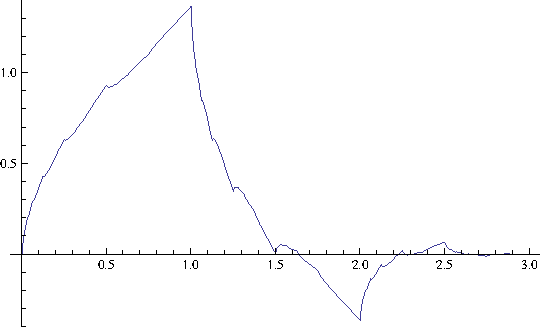
\includegraphics[width=\linewidth]{plaatjes/db2_phi.pdf}
  \end{subfigure}
  \begin{subfigure}{0.48\linewidth}
    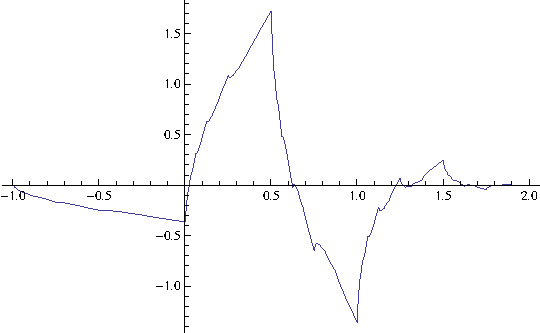
\includegraphics[width=\linewidth]{plaatjes/db2_psi.pdf}
  \end{subfigure}
  \caption{Links: de Daubechies-2 schalingsfunctie. Rechts: de Daubechies-2 waveletfunctie.}
\end{figure}

\section{Fast Wavelet Transform}

Door de recursieve relatie van de ruimtes in \ref{ruimterec} herhaald toe te passen,
kunnen we de ruimte $V_j$ schrijven in termen van $V_0$ en een scala aan
orthogonaal-complementsruimtes $W_k$.
\begin{equation}
  \label{ruimte_splitsing}
  V_j = V_k \oplus W_k \oplus \cdots \oplus W_{j-1} = \ldots
  = V_0 \oplus W_0 \oplus \cdots \oplus W_{j-1}
\end{equation}
We willen nu een functie $f$ benaderen in de ruimte $V_j$ door $P_{V_j}f$ te schrijven in
de basis van de ruimtes $V_0$ en de verschillende $W_k$. Hiervoor dienen we de inproducten
te bereken van $f$ met de basisvectoren in deze ruimtes.
We onderscheiden dan de \emph{approximatie}
co\"efficienten $a_j[n]$ en de \emph{detail} co\"efficienten $d_j[n]$, die
$f$ geven als projectie op  respectievelijk $V_j$ en $W_j$.

Het is echter veel rekenwerk om al deze co\"efficienten uit te rekenen, dit gebeurt immers
door het berekenen van integralen. We beperken ons daarom tot her uit rekenen van de
co\"efficienten op het niveau $j$ en proberen vervolgens een recursieve relatie te vinden
om hieruit de approximatie en detailco\"efficienten te vinden.

Vanwege de relatie in \ref{ruimterec} kunnen we de basisfuncties uit de ruimtes $W_{j-1}$,
$V_{j-1}$ schrijven in termen van de basisfuncties van de ruimte $V_j$.
We schrijven daarvoor $\phi_{j-1,n}$ om in termen van de basisfuncties $\phi_{j,k}$; evenzo
voor $\psi_{j-1,n}$.
\begin{equation}
  \label{phi_rec}
  \phi_{j-1,n} = \sum_{k=-\infty}^{\infty} \inpr{\phi_{j-1,n}}{\phi_{j,k}} \phi_{j,k}
\end{equation}
\begin{equation}
  \label{psi_rec}
  \psi_{j-1,n} = \sum_{k=-\infty}^{\infty} \inpr{\psi_{j-1,n}}{\phi_{j,k}} \phi_{j,k}
\end{equation}
We rekenen vervolgens de inproducten uit om deze om te schrijven naar een filterco\"efficient,
bekijk
\eq{
  \inpr{\phi_{j-1,n}}{\phi_{j,k}}
  =& \int_{-\infty}^\infty \sqrt{2^{j-1}}\phi(2^{j-1}t -n)
  \sqrt{2^{j}}\phi^\star(2^j t - k) \d{t}\\
  =& \int_{-\infty}^\infty \tfrac{1}{2^j} 2^{j-1}
  \sqrt{2} \phi(t') \phi(2t' - k + 2n) \d{t'}\\
  =& \inpr{\phi(t)}{\sqrt{2}\phi(2t-k+2n)} \\
  =& h[k-2n],
}
\eq{
  \inpr{\psi_{j-1,n}}{\phi_{j,k}}
  =& \int_{-\infty}^\infty \sqrt{2^{j-1}}\psi(2^{j-1}t -n)
  \sqrt{2^{j}}\phi^\star(2^j t - k) \d{t}\\
  =& \int_{-\infty}^\infty \tfrac{1}{2^j} 2^{j-1}
  \sqrt{2} \psi(t') \phi(2t' - k + 2n) \d{t'}\\
  =& \inpr{\psi(t)}{\sqrt{2}\phi(2t-k+2n)} \\
  =& g[k-2n],
}
waarbij we de co\"ordinaat-transformatie $t' = 2^{j-1}t - n$ hebben gebruikt.
Door nu aan beide zijden van vergelijkingen \ref{phi_rec}, \ref{psi_rec} het
inproduct met $f$ te nemen kunnen we de coe\"fficienten van de resolutie $2^{j-1}$ schrijven
in termen van de coe\"fficienten op de resolutie $2^j$.
\begin{equation}
  \label{approx_rec}
  a_{j-1}[n] = \inpr{f}{\phi_{j-1,n}}
  = \sum_{k=-\infty}^{\infty} h[k-2n] \inpr{f}{\phi_{j,k}}
  = \sum_{k=-\infty}^\infty h[k-2n] a_{j}[k]
  = (a_j \star \bar h)[2n]
\end{equation}
\begin{equation}
  \label{detail_rec}
  d_{j-1}[n] = \inpr{f}{\psi_{j-1,n}}
  = \sum_{k=-\infty}^{\infty} g[k-2n] \inpr{f}{\phi_{j,k}}
  = \sum_{k=-\infty}^\infty g[k-2n] a_{j}[k]
  = (a_j \star \bar g)[2n]
\end{equation}
Waarbij $\bar f: x \mapsto f(-x)$ en $x\star y$ de discrete convolutie aangeeft,
als kortere schrijfwijze van deze sommatie.
De relatie die hier gevonden is geeft aanleiding tot een algoritme.

\begin{algo}[Fast Wavelet Transform]
  Gegeven een rij co\"effici\"enten $a_j\in\R^{2^j}$ dan definie\"eren we een recursief
  algoritme $\mathrm{FWT}:\R^{2^j}\to\R^{2^j}$ volgens:\\
  Als $j=0$ dan geldt
  \[
  \mathrm{FWT}(a_j)[n] = a_j[n]
  \]
  Als $j>0$ bereken $a_{j-1}$ en $d_{j-1}$ volgens \ref{approx_rec}, \ref{detail_rec}.
  Vervolgens geldt
  \begin{equation}
    \label{FWT_cases}
    \mathrm{FWT}(a_j)[n] = \begin{cases}
      \mathrm{FWT}(a_{j-1})[n] & \text{als } n\leq 2^{j-1} \\
      d_{j-1}[n] & \text{als } n>2^{j-1} \end{cases}
  \end{equation}
\end{algo}
We gaan hierbij uit van een eindige filter en beschouwen onze ruimte $V_j$ als functies
op een interval in $\R$, dan versimpelen de oneindige sommaties in \ref{approx_rec},
\ref{detail_rec}. Voor een discrete functie $f\in\R^{2^j}$ kunnen we nu
$\mathrm{FWT}(f)$ nemen als de fast wavelet transform,
we nemen dan aan dat $\inpr{f}{a_{j,k}} = f[k]$ voor het
grootste niveau $V_j$. Deze aannames komen ruwweg neer op de bewering dat
$V_0 = \{\phi_{0,0}\}$ en dat zowel $\phi$ als $\psi$ een compacte drager heeft.

We kunnen vervolgens de transformatie inverteren aan de hand van het volgende algoritme
\begin{algo}[Inverse Fast Wavelet Transform]
  Gegeven een rij co\"effici\"enten $x_j\in\R^{2^j}$ dan definie\"eren we een recursief
  algoritme $\mathrm{iFWT}:\R^{2^j}\to\R^{2^j}$ volgens:\\
  Als $j=0$ dan geldt
  \[
  \mathrm{iFWT}(x_j)[n] = x_j[n]
  \]
  Als $j>0$ laat $x_{j-1}[n] = x_j[n]$ en $d_{j-1}[n] = x_j[n+2^{j-1}]$ voor
  $1\leq n\leq 2^{j-1}$. Bereken hiermee $a_{j-1} = iFWT(x_{j-1})$,
  dan geldt
  \begin{equation}
    \label{reconstr_FWT}
    \mathrm{iFWT}(x_j)[n] = (\breve a_{j-1}\star h)[n] + (\breve d_{j-1}\star g)[n]
  \end{equation}
  Waarbij $\breve y [2n] = y[n]$ en $\breve y [2n+1] = 0$.
\end{algo}
\begin{stelling}
  De iFWT (links) samengesteld met de FWT geeft de identiteit voor een signaal.
\end{stelling}
\begin{proof}[Bewijs]
  We bekijken de verschillende gevallen.Voor het geval $j=0$ geldt duidelijk dat
  \[
  \mathrm{iFWT}(\mathrm{FWT}(a_0)) = \mathrm{iFWT}(a_0) = a_0.
  \]
  We zullen dus verder moeten bewijzen dat \ref{reconstr_FWT} een inverse vormt voor
  \ref{FWT_cases}.
  Schrijf hiervoor de basisfuncties van $V_j$ in termen van de basisfuncties van $V_{j-1}$
  en $W_{j-1}$, ofwel:
  \[
  \phi_{j,n} = \sum_{k=-\infty}^\infty \inpr{\phi_{j,n}}{\phi_{j-1,k}}\phi_{j-1,k}
  + \sum_{-\infty}^\infty \inpr{\phi_{j,n}}{\psi_{j-1,k}}\psi_{j-1,k}
  \]
  Deze inproducten komen weer overeen met de filterco\"efficienten, nemen we dus aan
  beide zeiden het inproduct dan volgt
  \[
  a_j[n] = \sum_{k=-\infty}^\infty h[n-2k]a_{j-1}[k]
  + \sum_{-\infty}^\infty g[n-2k]d_{j-1}[k]
  \]
  Door nu in de sommatie de variabele $k$ te vervangen door $k'=2k$ vereenvoudigt dit tot
  \[
  a_j[n] = \sum_{k'=-\infty}^\infty h[n-k']\breve a_{j-1}[k']
  + \sum_{-\infty}^\infty g[n-2k]\breve d_{j-1}[k']
  \]
  Daarmee geeft de iFWT een inverse voor de FWT.
\end{proof}
\section{Analyse van de Wavelettransformatie}
Met de theoretische beschouwing van wavelets en de Fast Wavelet Transform achter de rug, kunnen we wat verder kijken naar practische obstakels.

\subsection{Eindige signalen}
Een van de eerste aannames die we tot nu toe steeds maakten is die van de oneindige signalen. Wanneer echter de functie $f$ een compacte drager heeft, worden een aantal zaken wat lastiger. Neem als eerste aan dat de drager van $f$ gewoon $[0,1]$ is.\footnote{Door translatie en dilatie kan elk signaal met compacte basis omgevormd worden tot een signaal met drager in $[0,1]$. We verliezen hier dus geen algemeenheid.} In dit geval zou het kunnen dat de waveletfuncties met een drager die $t=0$ of $t=1$ doorsnijdt, niet meer de gewenste eigenschappen heeft. Er zijn in de literatuur oplossingen voor dit probleem gevonden. Hier zullen wij verder niet op in gaan.

Wanneer we nu een benadering van $f$ maken op resolutie $2^J$ (door bijvoorbeeld een Fast Wavelet Transform), bekijken we
\[
V_0 \subset V_{1} \subset \ldots \subset V_{J}.
\]
Een discreet signaal van lengte $2^{J}$ kan zo perfect getransformeerd worden in een waveletbasis op resolutie $2^{J}$. Dit is precies waarom de Fast Wavelet Transform zo veel gebruikt wordt bij het analyseren van discrete signalen.

\subsection{Signaaluitbreiding}
Een probleem waar we in het geval van eindige signalen nog meer mee te maken krijgen is dat de algoritme niet goed omgaat met de randen. De convolutie moet nu ineens \emph{buiten het definitiegebied} van het signaal `kijken'. Eerder in sectie \ref{signaal} hebben we al gezien hoe signalen naar een tweemacht uitgebreid kunnen worden. Precies dezelfde methoden kunnen gebruikt worden om het signaal nog verder uit te breiden.

Om niet te veel tijd te verliezen met het ondersteunen van meerdere mogelijkheden hebben wij er voor gekozen om \emph{periodic padding} op alle signalen toe te passen. Dit omdat de zogenaamde \emph{circulaire convolutie} ingebouwd zit in de bibliotheek die wij gebruikt hebben.

\subsection{Complexiteit van de algoritme}
NOOT: rob heeft hier "nog niet" staan. wat?
Als de lengte van de filter $h$ gelijk is aan $K$, en de lengte van het originele signaal $a_L$ gelijk is aan $N = 2^{L}$, kunnen we voor $j \in \{0, \ldots, L\}$ zien dat $a_j$ en $d_j$ beide $2^{j}$ elementen bevatten. Nu kunnen $a_{j-1}$ en $d_{j-1}$ gemaakt worden door $2^{j}K$ operaties zodat elke stap van de algoritme $2^{j} \cdot K$ operaties kost. Dan kost het hele algoritme
\[
\sum_{j=L}^0 2^{j} \cdot K = K \sum_{j=L}^0 2^{j} = K \cdot (2^{1+L} - 1) < 2 \cdot K 2^{L} = 2KN
\]
operaties. Dus deze DWT is een $\mathcal{O}(KN)$ algoritme. Ook de complexiteit van de inverse wordt op dezelfde manier van orde $KN$.

\section{Meer dimensies: de Mallatdecompositie}
NOOT: meer stressen dat je een algemene vorm hebt die 2 decomposities geeft

Met een orthonormale waveletbasis $\{ \psi_{j,n}: (j,n) \in \Z^2\}$ van $L_2(\R)$ volgt een natuurlijke voortzetting naar twee dimensies door
\[
\{ \psi_{j_1,n_1}(x_1) \psi_{j_2,n_2}(x_2): (j_i,n_i) \in \Z^4 \},
\]
welke een orthonormale basis voor $L_2(\R^2)$ is. We zien direct dat we op de $x_1$-as met resolutie $2^{j_1}$ kijken terwijl de $x_2$-as resolutie $2^{j_2}$ kent.

Mallat vond dit iets om te vermijden \cite[\S 7.7]{mallat} en legt in zijn analyse dan ook de eis $j_1 = j_2 =: j$ op. Wij zullen in het vervolg \'o\'ok kijken naar het zogenaamde Tensorproduct, wat de eis $j_1 = j_2$ \emph{niet} oplegt.

Zoals in 1 dimensie is de notie van `resolutie' geformaliseerd in het begrip multiresolutie. De definitie van deze multiresolutie is wederom een natuurlijke voortzetting van het eendimensionale geval. Wanneer we spreken over een separeerbare multiresolutie, gaat het om een ruimte $V_j^{(2)} := V_j \otimes V_j$. In \cite[A.5]{mallat} wordt nu bewezen dat, gegeven een orthonormale basis $\{ \phi_{j,m}: m \in \Z \}$ voor $V_j$, de verzameling
\begin{equation}
  \label{phi_phi_basis}
  \{ \phi^{(2)}_{j,n} := \phi_{j,n_1} \otimes \phi_{j,n_2}: n \in \Z^2 \}
\end{equation}
een orthonormale basis voor $V_j^{(2)}$ is.

\begin{voorbeeld}
Bekijk weer $V_j$ de ruimte van stuksgewijs constante functies op het interval 
\[
 [2^{-j} m, 2^{-j}(m+1) ), m \in \Z.
\] 
We vinden voor $V_j^{(2)}$ nu de ruimte van stuksgewijs constante functies op vierkanten $[2^{-j}n_1, 2^{-j}(n_1+1)) \times [2^{-j}n_2, 2^{-j}(n_2+1))$. De tweedimensionale schalingsfunctie wordt op die manier
\[
	\phi^{(2)}(x_1,x_2) = \phi(x_1)\phi(x_2) = \begin{cases} 1 & \text{ als } x_1 \in [0,1)\text{ en }x_2 \in [0,1) \\ 0 & \text{ anders.} \end{cases}
\]
\end{voorbeeld}

\subsection{Tweedimensionale Waveletfuncties}
We weten dat $V_j^{(2)}$ bevat is in $V_{j+1}^{(2)}$. Bekijk het orthogonale complement $\boldsymbol{U}_j \perp V_j^{(2)}$:
\begin{equation}
  \label{2d_ruimte_rec}
  V_j^{(2)} \oplus \boldsymbol{U}_j = V_{j+1}^{(2)}.
\end{equation}
Om nu een orthogonale waveletbasis voor $\boldsymbol{U}_j$ en (dus in de limiet) $L^2(\R^2)$ te vinden, gaan we als volgt te werk.
\begin{stelling}[{\cite[T7.24]{mallat}}]
  Laat $\phi$ een schalingsfunctie en $\psi$ de bijhorende wavelet die en basis voor de $L^2(\R)$ voortbrengt. Maak drie wavelets
  \begin{equation}
    \label{psi_k_defs}
    \psi^1(x) = \phi(x_1)\psi(x_2) \quad \psi^2(x) = \psi(x_1) \phi(x_2) \quad \psi^3(x) = \psi(x_1)\psi(x_2)
  \end{equation}
  en laat voor $k \in \{1,2,3\}$ nu
  \[
  \psi^k_{j,n}(x) = 2^j \psi^k\left( 2^jx_1 - n_1, 2^j x_2 - n_2 \right).
  \]

  Dan is
  \[
  \{ \psi^1_{j,n}, \psi^2_{j,n}, \psi^3_{j,n}: n \in \Z^2 \}
  \] een basis voor $\boldsymbol{U}_j$
  en
  \[
  \{ \phi_{0, n}^2: n \in \Z^2 \} \cup \{ \psi^1_{j,n}, \psi^2_{j,n}, \psi^3_{j,n}: n \in \Z^2, j \in \N_0 \}
  \] een basis voor $L^2(\R^2)$.
\end{stelling}
\begin{proof}[Bewijs]
  We weten
  \[
  V_{j+1}^{(2)} = V_j^{(2)} \oplus \boldsymbol{U}_j \implies V_{j+1} \otimes V_{j+1} = ( V_j \otimes V_j ) \oplus \boldsymbol{U}_j.
  \]
  Vul nu $V_{j+1} = V_j \oplus W_j$ in om te vinden
  \[
  ( V_j \oplus W_j ) \otimes (V_j \oplus W_j ) = (V_j \otimes V_j) \oplus \boldsymbol{U}_j
  \]
  \[
  \implies (V_j \otimes V_j) \oplus (V_j \otimes W_j) \oplus (W_j \otimes V_j) \oplus (W_j \otimes W_j) = (V_j \otimes V_j) \oplus \boldsymbol{U}_j
  \]
  \[
  \implies (V_j \otimes W_j) \oplus (W_j \otimes V_j) \oplus (W_j \otimes W_j) = \boldsymbol{U}_j.
  \]
  Nu is het duidelijk dat $\{ \psi^1_{j,n}, \psi^2_{j,n}, \psi^3_{j,n}: n \in \Z^2 \}$ een basis is voor $\boldsymbol{U}_j$.

Omdat nu via vergelijking \ref{ruimterec} moet gelden
\[
	L^2(\R^2) = \lim_{j \to \infty} V_j^{(2)} = \lim_{j \to \infty} ( V_0^{(2)} \oplus \boldsymbol{U}_0 \oplus \cdots \oplus \boldsymbol{U}_{j-1} ) = \left( \bigoplus_{j=0}^\infty \boldsymbol{U}_j \right) \oplus V_0^{(2)}
\]
is $\{ \phi_{0, n}^2: n \in \Z^2 \} \cup \{ \psi^1_{j,n}, \psi^2_{j,n}, \psi^3_{j,n}: n \in \Z^2, j \in \N_0 \}$ een basis voor $L^2(\R^2)$.
\end{proof}
\begin{gevolg}
In het bewijs wordt nu ook duidelijk dat 
\[
	\left\{ \phi_{0, n}^2: n \in \Z^2 \right\} \cup \left\{ \psi^1_{j,n}, \psi^2_{j,n}, \psi^3_{j,n}: n \in \Z^2, j \in \{0, \ldots, L \}  \right\}
\]
een basis voor $V_L^{(2)}$ is.
\end{gevolg}

Bovenstaande basis heeft dus schalingsfuncties op \'e\'en niveau en waveletfuncties op alle niveaus. Net zoals in het eendimensionale geval kunnen we met deze basis een algoritme formuleren.

\subsection{Naar een tweedimensionaal algoritme}
Nu we een relatie hebben gevonden $(\ref{2d_ruimte_rec})$ tussen de ruimtes op verschillende
niveau's volgens
\begin{equation}
  \label{2d_ruimte_decomp}
V_{j+1}^{(2)} = (V_j\otimes W_j) \oplus (W_j\otimes V_j) \oplus
(W_j\otimes W_j) \oplus (V_j\otimes V_j)
\end{equation}
kunnen we het eendimensionale algoritme uitbreiden naar twee dimensies.
Hiervoor kijken we wederom naar de inproducten van een functie $f$ met
onze basisfuncties.
We defini\"eren daarvoor weer de \emph{approximatie}~co\"effici\"ent en een drietal
van \emph{detail}~co\"effici\"enten volgens.
\[
a_j[n] := \langle f, \phi^{(2)}_{j,n} \rangle \quad d^k_j[n] := \langle f, \psi^k_{j,n} \rangle ,\quad k \in \{1,2,3\}.
\]
We zullen nu in het bijzonder kunnen zeggen (maak gebruik van $\ref{phi_phi_basis}$)
dat we de basis-functies op het niveau $j$ kunnen ontbinden volgens:
\begin{equation}
  \label{phi_phi_som}
  \phi^{(2)}_{j,(n_1,n_2)} = \sum_{k_1=-\infty}^\infty \sum_{k_2=-\infty}^\infty
  \inpr{\phi_{j,n_1}\otimes\phi_{j,n_2}}{\phi_{j+1,k_1}\otimes\phi_{j+1,k_2}}
  \phi^{(2)}_{j+1,(k_1,k_2)}
\end{equation}
\begin{equation}
  \label{psi_k_som}
  \psi^{p}_{j,(n_1,n_2)} = \sum_{k_1=-\infty}^\infty \sum_{k_2=-\infty}^\infty
  \inpr{\psi^p_{j,(n_1,n_2)}}{\phi_{j+1,k_1}\otimes\phi_{j+1,k_2}}
  \phi^{(2)}_{j+1,(k_1,k_2)}
\end{equation}
We maken nu gebruik van \emph{TODO ref} om het inproduct behorende bij het tensorproduct
van twee \emph{Hilbertruimten} uit te schrijven volgens:
\[
\inpr{a\otimes b}{c\otimes d} = \inpr{a}{c}\cdot \inpr{b}{d}
\]
Waarbij de inproducten lopen over de respectievelijke ruimtes.
Dit versimpelt de inproducten die we zoeken volgens:
\[
\inpr{\phi_{j,n_1}\otimes\phi_{j,n_2}}{\phi_{j+1,k_1}\otimes\phi_{j+1,k_2}}
=\inpr{\phi_{j,n_1}}{\phi_{j+1,k_1}}\inpr{\phi_{j,n_2}}{\phi_{j+1,k_2}}
=h[k_1-2n_1]\cdot h[k_2-2n_2]
\]
Waarbij we de filterrelatie voor \'e\'en dimensie toepassen. We kunnen dit nog een
stuk verbeteren door het product $h[\_]\cdot h[\_]$ om te schrijven naar een tensorproduct,
dan is:
\[
h\otimes h : \Z\times\Z \to \R :: (x_1,x_2) \mapsto h[x_1]\cdot h[x_2]
\]
Deze stappen kunnen nu ook met hetzelfde argument toegepast worden op de $\psi^k$'s,
we verkrijgen dan met een blik op de definities in ($\ref{psi_k_defs}$) de vergelijkingen:
\[
\inpr{\psi^1_{j,(n_1,n_2)}}{\phi^{(2)}_{j+1,(k_1,k_2)}} = (h\otimes g) [k_1-2n_1,k_2-2n_2]
\]
\[
\inpr{\psi^2_{j,(n_1,n_2)}}{\phi^{(2)}_{j+1,(k_1,k_2)}} = (g\otimes h) [k_1-2n_1,k_2-2n_2]
\]
\[
\inpr{\psi^3_{j,(n_1,n_2)}}{\phi^{(2)}_{j+1,(k_1,k_2)}} = (g\otimes g) [k_1-2n_1,k_2-2n_2]
\]
We richten ons nu weer op de \emph{approximatie} en \emph{detail}~co\"effici\"enten door
aan beide zeiden van de vergelijkingen $\ref{phi_phi_som}$,$\ref{psi_k_som}$ het inproduct
met $f$ te nemen. We kunnen dit aan de hand van onze nieuwe 2-dimensionale filters
opschrijven met een convolutie in twee dimensies, namelijk
\begin{eqnarray}
  \label{2d_coef_rec}
  a_{j}[n_1,n_2] =& (a_{j+1} \star (\bar{h} \otimes \bar{h}))[2n_1,2n_2] \\
  d^1_{j}[n_1,n_2] =&( a_{j+1} \star (\bar{h} \otimes \bar{g}))[2n_1,2n_2] \\
  d^2_{j}[n_1,n_2] =& (a_{j+1} \star (\bar{g} \otimes \bar{h}))[2n_1,2n_2] \\
  \label{2d_coef_rec_last}
  d^3_{j}[n_1,n_2] =& (a_{j+1} \star (\bar{g} \otimes \bar{g}))[2n_1,2n_2]
\end{eqnarray}
waarbij de convolutie gegeven wordt door
\[
(x \star y)[n_1,n_2] := \sum_{p_1=-\infty}^\infty \sum_{p_2 = -\infty}^\infty
x[n_1 - p_1,n_2 - p_2] \cdot y[n_1-p_1, n_2 - p_2].
\]


\begin{algo}[Tweedimensionale Fast Wavelet Transform]
  Gegeven een matrix van co\"effici\"enten $a_j\in\R^{2^j}\times\R^{2^j}$ dan definie\"eren
  we een recursief algoritme $\mathrm{FWT}_2:\R^{2^j}\times\R^{2^j}\to\R^{2^j}\times\R^{2^j}$
  volgens:\\
  Als $j=0$ dan geldt
  \[
  \mathrm{FWT}_2(a_j)[n_1,n_2] = a_j[n_1,n_2]
  \]
  Als $j>0$ bereken $a_{j-1}$,$d^1_{j-1}$,$d^2_{j-1}$ en $d^3_{j-1}$ uit $a_{j}$
  volgens $(\ref{2d_coef_rec}-\ref{2d_coef_rec_last})$
  Vervolgens geldt
  \begin{equation}
    \label{FWTd_def}
  \mathrm{FWT}_2(a_j)[n_1,n_2] = \begin{cases}
    \mathrm{FWT}_2(a_{j-1})[n_1,n_2] & \text{als } n_1 \leq 2^{j-1} \text{ en } n_2 \leq 2^{j-1}\\
    d^1_{j-1}[n_1,n_2]
    & \text{als } n_1\leq 2^{j-1} \text{ en } n_2>2^{j-1} \\
    d^2_{j-1}[n_1,n_2]
    & \text{als } n_1>2^{j-1} \text{ en } n_2\leq 2^{j-1} \\
    d^3_{j-1}[n_1,n_2] & \text{als } n_1>2^{j-1} \text{ en } n_2>2^{j-1} \end{cases}
  \end{equation}
\end{algo}
\begin{algo}[Inverse Tweedimensionale Fast Wavelet Transform]
  Gegeven een matrix van  co\"effici\"enten $x_j\in\R^{2^j}\times\R^{2^j}$ dan definie\"eren we hierop het recursieve
  algoritme $\mathrm{iFWT}_2:\R^{2^j}\times\R^{2^j}\to\R^{2^j}\times\R^{2^j}$ volgens:\\
  Als $j=0$ dan geldt
  \[
  \mathrm{iFWT}_2(x_j)[n_1,n_2] = x_j[n_1,n_2]
  \]
  Als $j>0$, splits dan $x_j$ in zijn vier kwadranten; laat voor $k_1,k_2\in \{1,\ldots,2^{j-1}\}$
  \begin{eqnarray*}
    y_{j-1}[k_1,k_2]   =& x_j[k_1,k_2] \\
    d^1_{j-1}[k_1,k_2] =& x_j[k_1,k_2+2^{j-1}] \\
    d^2_{j-1}[k_1,k_2] =& x_j[k_1+2^{j-1},k_2] \\
    d^3_{j-1}[k_1,k_2] =& x_j[k_1+2^{j-1},k_2+2^{j-1}]
  \end{eqnarray*}
  Bereken hiermee vervolgens $a_{j-1} = \mathrm{iFWT}_2(y_{j-1})$,
  dan geldt
  \begin{equation}
    \label{iFWTd_def}
    \begin{split}
      \mathrm{iFWT}_2(a_j)[n_1,n_2] =& \breve{a}_{j-1} \star (h \otimes h)[n_1,n_2] 
      + \breve{d}_{j-1}^1 \star (h \otimes g)[n_1,n_2] \\
      +& \breve{d}_{j-1}^2 \star (g \otimes h)[n_1,n_2] 
      + \breve{d}_{j-1}^3 \star (g \otimes g)[n_1,n_2]
    \end{split}
  \end{equation}
  Waarbij 
  \[
  \breve y [n_1,n_2] = \begin{cases} 
    y[n_1/2,n_2/2] & \text{als } 2|n_1 \text{ en } 2|n_2 \\ 
    0 &\text{anders}\end{cases}
  \]
\end{algo}
\begin{stelling}
  De $\mathrm{iFWT}_2$ (links) samengesteld met de $\mathrm{FWT}_2$ geeft de identiteit voor een signaal.
\end{stelling}
\begin{proof}[Bewijs]
  We bekijken de verschillende gevallen. Voor het geval $j=0$ geldt duidelijk dat
  \[
  \mathrm{iFWT}_2(\mathrm{FWT}_2(a_0)) = \mathrm{iFWT}_2(a_0) = a_0.
  \]
  Voor het geval $j>0$ merken we op dat wanneer de $\mathrm{iFWT}_2$ werkt voor $j'<j$ de co\"effici\"enten-matrices
  $a,d^1,d^2,d^3$ precies zijn wat de $\mathrm{FWT}_2$ zou geven op dit niveau. 
  We zullen dus verder moeten bewijzen dat \ref{iFWTd_def} een inverse vormt voor
  \ref{FWTd_def}.
  Schrijf hiervoor de basisfuncties van $V^{(2)}_j$ in termen van de basisfuncties van 
  $V_{j-1}\otimes V_{j-1}$, $V_{j-1}\otimes W_{j-1}$, $W_{j-1}\otimes V_{j-1}$ en $W_{j-1}\otimes W_{j-1}$
  dit is geoorloofd zoals we gezien hebben in een vorige sectie.
  \begin{equation*}
    \begin{split}
      \phi_{j,(n_1,n_2)} = 
      \sum_{k_1=-\infty}^\infty\sum_{k_2=-\infty}^\infty 
      \inpr{\phi^{(2)}_{j,(n_1,n_2)}}{\phi^{(2)}_{j-1,(k_1,k_2)}} \phi^{(2)}_{j-1,(k_1,k_2)} \\
      + \sum_{k_1=-\infty}^\infty\sum_{k_2=-\infty}^\infty 
      \inpr{\phi^{(2)}_{j,(n_1,n_2)}}{\psi^1_{j-1,(k_1,k_2)}} \psi^1_{j-1,(k_1,k_2)} \\
      + \sum_{k_1=-\infty}^\infty\sum_{k_2=-\infty}^\infty 
      \inpr{\phi^{(2)}_{j,(n_1,n_2)}}{\psi^2_{j-1,(k_1,k_2)}} \psi^2_{j-1,(k_1,k_2)} \\
      + \sum_{k_1=-\infty}^\infty\sum_{k_2=-\infty}^\infty 
      \inpr{\phi^{(2)}_{j,(n_1,n_2)}}{\psi^3_{j-1,(k_1,k_2)}} \psi^3_{j-1,(k_1,k_2)}
      \end{split}
  \end{equation*}
  Deze inproducten tussen basisfuncties komen weer overeen met de filterco\"efficienten. Nemen we dus aan
  beide zeiden het inproduct met $f$ dan volgt de vergelijking voor de approximatie-co\"effici\"enten
  \begin{equation*}
    \begin{split}
      a_{j}[n_1,n_2] = 
      \sum_{k_1=-\infty}^\infty\sum_{k_2=-\infty}^\infty 
      (h\otimes h)[n_1-2k_1,n_2-2k_2] a_{j-1}[k_1,k_2] \\
      + \sum_{k_1=-\infty}^\infty\sum_{k_2=-\infty}^\infty 
      (h\otimes g)[n_1-2k_1,n_2-2k_2] d^1_{j-1}[k_1,k_2] \\
      + \sum_{k_1=-\infty}^\infty\sum_{k_2=-\infty}^\infty 
      (g\otimes h)[n_1-2k_1,n_2-2k_2] d^2_{j-1}[k_1,k_2] \\
      + \sum_{k_1=-\infty}^\infty\sum_{k_2=-\infty}^\infty 
      (g\otimes g)[n_1-2k_1,n_2-2k_2] d^3_{j-1}[k_1,k_2]
      \end{split}
  \end{equation*}
  Door nu in de sommatie de variabelen $k_1,k_2$ te vervangen door $k_1'=2k_1$ respectievelijk $k_2'=2k_2$ 
  vereenvoudigt dit tot
  \begin{equation*}
    \begin{split}
      a_{j}[n_1,n_2] = 
      \sum_{k_1'=-\infty}^\infty\sum_{k_2'=-\infty}^\infty 
      (h\otimes h)[n_1-k_1',n_2-k_2'] \breve a_{j-1}[k_1',k_2'] \\
      + \sum_{k_1'=-\infty}^\infty\sum_{k_2'=-\infty}^\infty 
      (h\otimes g)[n_1-k_1',n_2-k_2'] \breve d^1_{j-1}[k_1',k_2'] \\
      + \sum_{k_1'=-\infty}^\infty\sum_{k_2'=-\infty}^\infty 
      (g\otimes h)[n_1-k_1',n_2-k_2'] \breve d^2_{j-1}[k_1',k_2'] \\
      + \sum_{k_1'=-\infty}^\infty\sum_{k_2'=-\infty}^\infty 
      (g\otimes g)[n_1-k_1',n_2-k_2'] \breve d^3_{j-1}[k_1',k_2']
      \end{split}
  \end{equation*}
  Wat precies gelijk is aan de convolutie in \ref{iFWTd_def}. Daarmee geeft de iFWT een inverse voor de FWT.
\end{proof}

\subsection{Meer dan twee dimensies}
Het $n$-dimensionale geval van de Mallatdecompositie is nog TODOOO

\subsection{Eindige signalen in $n$ dimensies}
De notie van eindige signalen is al eerder langsgekomen. We bekijken functies met een compacte drager $[0,1]$. Het gevolg hiervan is dat de complete waveletbasis teveel elementen bevat. Alleen wavelets waarvan de drager het interval doorsnijdt, zijn voor ons interessant. Wanneer we nu naar meer dimensies gaan, praten we over een $n$-dimensionaal eenheidsinterval $[0,1]^n =: \Box$. 

\iffalse
Zoals in een eerdere sectie in 1 dimensie al aan werd gegeven, kijken we in de praktijk vaak naar signalen met een compacte drager, zeg $\Box := [0,1]^n$. Dan focussen we ons dus op functies $f \in L_2(\Box)$ en niet meer op functies in $L_2(\R^n)$. Net zoals eerder komen er problemen voor wavelets `op de rand'. Wij zullen hier wederom geen verdere aandacht aan besteden.

Wanneer we $L_2(\Box)$ als deelruimte van $L_2(\R^n)$ beschouwen, is er een natuurlijke basis voor deze deelruimte te vinden. Neem namelijk alle basisfuncties met een drager die $\Box$ doorsnijdt (de rest is op $\Box$ namelijk gewoon de nulfunctie). Definieer $\nabla$ als de verzameling indices $\lambda := (j, n)$ van wavelets die drager doorsnijden met $[0,1]$. Dan wordt $\Psi := \{ \psi_\lambda: \lambda \in \nabla \}$ een basis voor $L_2([0,1])$. Definieer daarnaast $|\lambda| := |(j,n)| = j$ als het niveau.

NOOT: dit stukje is poep.


Concreet zullen we echter niet gebruik maken van signalen die leven in $L^2(\R^n)$. We zullen eerder op zoek zijn naar de Wavelettransformatie van een signaal met compacte drager. Neem dus aan dat $f$ leeft in $L^2([0,1]^n)$. Dit $n$-dimensionale eenheidsinterval wordt ook wel met $\Box$ aangegeven. Omdat $\Box \subset \R^n$, kunnen we een waveletbasis voor $L^2(\R^n)$ ook als basis nemen voor $L^2(\Box)$. Maar eigenlijk is dit iets te veel (gezien het feit dat veel basisfuncties hun drager geheel buiten het interval zullen hebben). Daarom wordt de verzameling van indices $\lambda := (j,n)$ van wavelets die drager doorsnijden met $[0,1]$ ook wel $\nabla$ genoemd. Dus $\Psi = \{ \psi_\lambda: \lambda \in \nabla \}$ wordt nu een basis voor $L^2([0,1])$. Defini\"eer $|\lambda| = |(j,n)| = j$ als het niveau.
Verder zullen we vanaf nu aannemen dat $\boldsymbol\psi$ een compacte drager heeft (zoals we in de praktijk altijd willen) en van orde $p$ is.
\fi

\section{Tensorproduct}
Herinner dat we voor de Mallat-decompositie gebruik maakte van de gelijkheid (zie \ref{2d_ruimte_decomp}):
\[
V_{j}^{(2)} = (V_{j-1}\otimes W_{j-1}) \oplus (W_{j-1}\otimes V_{j-1}) \oplus
(W_{j-1}\otimes W_{j-1}) \oplus (V^{(2)}_{j-1})
\]
Door dit herhaald toe te passen kregen we een basis van de vorm:
\[
\{\phi^{(2)}_{0,(n_11,n_2)}\largediv n_1,n_2\in\Z\}\cup
\{\psi^k_{j,(n_1,n_2)} \largediv k=1,2,3\quad j\in \N_0 \quad n_1,n_2\in\Z\}
\]
We zullen nu echter zien dat er ook een andere manier is om deze ruimte te decomposeren.
Bedenk dat we in 1 dimensie de decompositie zoals in \ref{ruimte_splitsing} gebruiken volgens:
\[
V_j = V_0 \oplus W_0 \oplus \cdots \oplus W_{j-1}
\]
Daarmee schrijven we de ruimte $V^{(2)}_j$ als het tensorproduct van $V_j$ met zichzelf:
\[
V^{(2)}_j = V_j\otimes V_j = (V_0\oplus W_0\oplus\cdots W_{j-1})\otimes(V_0\oplus W_0\oplus\cdots W_{j-1})
\]
Dit geeft aanleiding tot een nieuwe basis, namelijk het tensorproduct van de basis van $V_j$ met zichzelf,
we duiden deze basis dan ook aan als de \emph{Tensorbasis}.
\footnote{In de literatuur wordt de Mallatdecompositie ook regelmatig een Tensorproduct genoemd. 
De verwarring ontstaat hier doordat in de Mallat Basis de basisfuncties ook tensorproducten zijn van wavelet- 
en schalingsfuncties. We doelen echter in onze naamgeving op \emph{het tensorproduct van twee bases}.}
\begin{equation}
  \label{tensor_basis_def}
  \begin{split}
    \boldsymbol \Psi_T :=& (\{\phi_{0,n}\largediv n\in\Z\}\cup \{\psi_{j,n}\largediv j\in\N_0\quad n\in\Z\})^2\\
                        =& \{\phi_{0,n_1}\otimes\phi_{0,n_2}\largediv n_1,n_2\in\Z\} 
                        \cup \{\phi_{0,n_1}\otimes\psi_{j,n_2}\largediv j\in\N_0\quad n_1,n_2\in\Z\} \\    
                         & \cup \{\psi_{j,n_1}\otimes\phi_{0,n_2}\largediv j\in\N_0\quad n_1,n_2\in\Z\} \\
                         & \cup \{\psi_{j_1,n_1}\otimes\psi_{j_2,n_2}\largediv j_1,j_2\in\N_0\quad n_1,n_2\in\Z\} \\
  \end{split}
\end{equation}
Waar $A^2 = \{a\otimes b \largediv a,b\in A\}$ een tensorproduct van een basis met zichzelf geeft.

Een karakteristiek van de Mallatbasis is, dat deze $\psi \otimes \psi$ functies bevat van enkel dezelfde schaal,
bij de Tensorbasis hebben we nu $j_1$ en $j_2$ die ongelijk aan elkaar zijn.
De Mallatbasis moest door deze eis aangevuld worden met functies van de vorm $\phi\otimes\psi$ en $\psi\otimes\phi$,
dit is bij de Tensorbasis niet meer aan de orde (met uitzondering van enkele samenstellingen van $\phi_0$ met $\psi_j$'s)

We willen nu een algoritme bedenken dat een tweedimensionaal schrijft in termen van de Tensorbasis,
we zullen zien dat dit neerkomt op het uitvoeren van FWT op alle rijen en kolommen van de ingangssignaal (een matrix)

\begin{algo}[Tweedimensionale Tensor Fast Wavelet Transform]
Gegeven een ingangssignaal $a_j\in\R^{2^j}\times\R^{2^j}$ dan defini\"eren we een bijbehorend sequentieel algoritme 
$\mathrm{TFWT}_2:\R^{2^j}\times\R^{2^j}\to \R^{2^j}\times\R^{2^j}$ door het schema:\\
Bereken $\tilde a_j$ zo dat geldt:
\[
\tilde a_j[n_1,n_2] = \mathrm{FWT}(a_j\largediv_{x_1=n_1})[n_2] 
\]
Dan wordt de $\mathrm{TFWT}_2$ gegeven door:
\[
\mathrm{TFWT}_2(a_j)[n_1,n_2] = \mathrm{FWT}(\tilde a_j\largediv_{x_2=n_2})[n_1]
\] 
Waarbij de notatie $a\largediv_{x_i=c}$ staat voor de vector die verkregen wordt door uit $a$
de $i$'de co\"ordinaat vast te zetten (e.g. $a\largediv_{x_1=c}[d] = a[c,d]$).
\end{algo}

We zullen aantonen dat de $\mathrm{TFWT}_2$ ook inderdaad een decompositie geeft in termen van de Tensorbasis.
We zijn namelijk op zoek naar een matrix van de vorm:
\begin{equation}
\label{TFWT_mat}
\begin{bmatrix}
\inpr{f}{\phi_0\otimes\phi_0}     & \inpr{f}{\phi_0\otimes\psi_0}     & \cdots & \inpr{f}{\phi_0\otimes\psi_\lambda} \\
\inpr{f}{\psi_0\otimes\phi_0}     & \inpr{f}{\psi_0\otimes\psi_0}     & \cdots & \inpr{f}{\psi_0\otimes\psi_\lambda} \\ 
           \vdots                 &         \vdots                    & \ddots &                \vdots  \\ 
\inpr{f}{\psi_\lambda\otimes\phi_0} & \inpr{f}{\psi_\lambda\otimes\psi_0} 
& \cdots & \inpr{f}{\psi_\lambda\otimes\psi_\lambda} \\
\end{bmatrix}
\end{equation}
Waarbij $\lambda$ een index geeft over de interessante basisfuncties.
We weten nu dat wanneer we de FWT nemen in \'e\'en co\"ordinaat door de andere co\"ordinaat vast te nemen,
 dit ons voor elke vaste waarde een vector geeft volgens:
\[
y \mapsto
\begin{bmatrix}
\inpr{f\largediv_{x_2=y}}{\phi_0} & 
\inpr{f\largediv_{x_2=y}}{\psi_0} & \cdots & 
\inpr{f\largediv_{x_2=y}}{\psi_\lambda}
\end{bmatrix}
\]
Hieruit kunnen we ook een vector van functies maken door de rol van functie en matrix-index om te wisselen:
\[
\begin{bmatrix}
y \mapsto \inpr{f\largediv_{x_2=y}}{\phi_0} & 
y \mapsto \inpr{f\largediv_{x_2=y}}{\psi_0} & \cdots & 
y \mapsto \inpr{f\largediv_{x_2=y}}{\psi_\lambda}
\end{bmatrix}
\]
Wanneer we nu voor elke functie in deze vector de FWT bereken zullen we weer een vector inproducten krijgen
voor elke co\"ordinaat in de originele vector, schrijf deze vector van vectoren (equivalent met een matrix) uit als 
$M[\lambda_1,\lambda_2]$,
\footnote{Hier wordt het inproduct van $\phi_0$ weggelaten om de schrijfwijze te verduidelijken.}
dan volgt:
\[
M[\lambda_1,\lambda_2] = \inpr{y\mapsto \inpr{f\largediv_{x_2=y}}{\psi_{\lambda_1}}}{\psi_{\lambda_2}}
\]
We kunnen dit omschrijven door de definitie van het inproduct op functieruimten toe te passen:
\[
\inpr{y\mapsto \inpr{f\largediv_{x_2=y}}{a}}{b} = 
\int_{-\infty}^\infty\int_{-\infty}^\infty f(x_1,x_2) \cdot a(x_1) \d{x_1} \cdot b(x_2) \d{x_2} = \inpr{f}{a\otimes b} 
\]
Waardoor de matrix $M$ identiek is aan \ref{TFWT_mat}. 

Het vinden van een inverse voor dit algoritme is nu ook triviaal, de iFWT geeft samengesteld met de FWT
immers de identiteit, zodat het toepassen op kolommen en rijen van de iFWT de $\mathrm{TFWT}_2$ inverteert.

\subsection{Meer dan twee dimensies}
Er is nu een natuurlijke voortzetting van het Tensorproduct naar meerdimensionale signalen.
Dit doen we namelijk door voor bijvoorbeeld $n$ dimensies als basis voor $V^{(n)}_j$ de basis te kiezen die we verkrijgen 
door de basis van $V_j$ met tensorproducten tot de $n$-de macht te verheffen.
Vervolgens is het algoritme aan te passen zodat het steeds over \'e\'en co\"ordinaat de FWT uitvoert, 
met bijbehorende inverse.

Omdat de stap in complexiteit van de notatie vele male groter is dan de benodigde denkstap laten we hier een rigoreuze
behandeling van de meerdimensionale Tensor Fast Wavelet Transform achterwege.

\section{Analyse van de fout van beide decomposities}

Bij compressie is men op zoek naar een manier om stukjes data weg te kunnen gooien of te schrijven op zo'n manier dat het minder ruimte inneemt. Wij zijn in het bijzonder ge\"interesseerd naar \emph{hoe dichtbij} we bij perfecte reconstructie zitten wanneer we een vooraf bepaald aantal data opslaan. Er is al uitgebreid onderzoek gedaan naar hoe dit werkt bij de waveletbasis en een aantal resultaten hiervan zullen we opnemen in ons verslag.

Laat $f$ een functie in $L^2(\Box)$ met aftelbare orthonormale basis $\mathcal{B} = \{ g_m \}$. Dan valt $f$ in deze basis te schrijven als
\[
f = \sum_{m = 0}^\infty \langle f, g_m \rangle g_m.
\]

\begin{lemm}[Parsevalgelijkheid\cite{parseval}]
  Als nu een functie $f$ in $L^2(\Box)$ geschreven wordt in $\mathcal{B}$ dan geldt
  \[
  \|f\|^2 = \sum_{m=1}^\infty | \langle f, g_m \rangle |^2.
  \]
\end{lemm}
\begin{proof}[Bewijs]
  TODO: bewijs skippen, reference er in?
  We hebben te maken met een Hilbertruimte dus
  \[
  \|f\|^2 = \langle f, f \rangle = \left\langle \sum_{m=1}^\infty \langle f, g_m \rangle g_m, \sum_{n=0}^\infty \langle f, g_n \rangle g_n \right\rangle = \sum_{m=1}^\infty \sum_{n=0}^\infty \left\langle \langle f, g_m \rangle g_m, \langle f, g_n \rangle g_n \right \rangle
  \]
  \[
  = \sum_{m=1}^\infty \sum_{n=1}^\infty \langle f, g_m \rangle \overline{\langle f, g_n \rangle}\langle g_m, g_n \rangle = \sum_{m=1}^\infty \sum_{n=1}^\infty \langle f, g_m \rangle \overline{\langle f, g_n \rangle} \delta_{m,n}
  \]
  \[ = \sum_{m=1}^\infty \langle f, g_m \rangle \overline{\langle f, g_m \rangle} = \sum_{m=1}^\infty |\langle f, g_m \rangle |^2.
  \]
\end{proof}

\begin{gevolg}
\label{linfout}
Wanneer we nu niet de hele basis, maar zeg alleen de eerste $N$ elementen pakken, krijgen we een verzameling $\mathcal{B}_N \subset \mathcal{B}$ zodat
\[
f_{\mathcal{B}_N} := \sum_{m = 1}^N \langle f, g_m \rangle g_m.
\]

In het bijzonder zijn we nu op zoek naar de \emph{fout} $\| f - f_{\mathcal{B}_N} \|$:
\[
\| f - f_{\mathcal{B}_N} \|^2 = \left\| \sum_{m=1}^\infty\langle f, g_m \rangle g_m - \sum_{m=1}^N \langle f, g_m \rangle g_m \right\|^2 = \left\| \sum_{m=N+1}^\infty\langle f, g_m \rangle g_m \right\|^2 = \sum_{m=N+1}^\infty | \langle f, g_m \rangle |^2.
\]
Duidelijk moge zijn dat voor $N \to \infty$, $\| f - f_{\mathcal{B}_N} \|^2 \to 0$.
\end{gevolg}

\begin{definitie}[Sobolevruimte]
Een Sobolevruimte $H^p(\Omega)$ over $\Omega \subset \R^n$ is de verzameling van alle functies $u \in L_2(\Omega)$ z\'o dat voor elke $\alpha \in \R^n$ geldt dat $|\alpha| \leq p \implies D^\alpha u \in L_2(\Omega)$. De zwakke parti\"ele afgeleide $D^\alpha u$ betekent
\[
	D^\alpha u := \frac{\partial^{|\alpha|} u}{\partial x_1^{\alpha_1} \cdots \partial x_n^{\alpha_n} }.
\]

De norm op $H^p$ wordt nu
\[
	\| u \|_{H^p(\Omega)} := \sum_{|\alpha| \leq k} \| D^\alpha u \|_{L_2(\Omega)}.
\]
\end{definitie}

\subsection{Fout van de Mallatdecompositie}
NOOT: mallat-waveletbasis uitwerken/vermelden
Wij zijn op het moment ge\"interesseerd in de Mallat-waveletbasis $\boldsymbol\Phi$. Deze is ook duidelijk aftelbaar dus we kunnen gevolg~\ref{linfout} gebruiken. 

Defini\"eer $J_M := \{ l \in \N^n: \| l \|_\infty \leq M \}$. Laat $\boldsymbol\Phi_M := \{ \boldsymbol{\psi}_{\boldsymbol{\lambda}} \in \boldsymbol\Phi: |\boldsymbol\lambda| \in J_M \}$ met $|\boldsymbol\lambda| = (|\lambda_1, \ldots, |\lambda_n|)$ de verzameling basisfuncties tot een niveau $M$.

\begin{stelling}[Fout van Mallatdecompositie]
Wanneer $f \in H^p(\Box)$, zal de fout $\| f - f_{\mathcal{\boldsymbol\Phi}_M} \|$ bij een Mallatdecompositie met de basisfuncties tot niveau $M$ hoogstens proportioneel met $N^{-p/n}$ zijn, met $N := \# \boldsymbol\Phi_M$ het aantal basisfuncties tot niveau $M$.
\end{stelling}
\begin{proof}

  We maken gebruik van de zogenaamde Jacksonongelijkheid \cite{jackson} die zegt dat 
  \[
  \inf_{q \in \mathbb{P}_{p-1}} ||f - q||_{L_2(\Box)} \simeq 2^{-jp} ||f||_{H^p(\Box)}
  \]
  wanneer $f \in H^p(\Box)$.

  Voor elke dimensie zitten er $\mathcal{O}(2^M)$ basisfuncties in $\{ \psi_\lambda: |\lambda| \leq M \}$. Er zijn $n$ dimensies dus $2^{Mn} = N$ basisfuncties in totaal.

  Bekijk de fout:
  \[
  \left\| f - f_{\boldsymbol\Phi_M} \right\|^2_{L_2(\Box)} = \sum_{{\boldsymbol\psi} \in \boldsymbol\Phi \setminus \boldsymbol\Phi_M} | \langle f, \boldsymbol\psi \rangle |^2 \simeq \sum_{|\boldsymbol\lambda| > M} 2^{-|\boldsymbol\lambda|p} \simeq 2^{-Mp},
  \]
  waarbij het laatste isteken voortkomt uit
  \[
  \sum_{k=M+1}^\infty 2^{- kp} = \frac{2^{-Mp}}{2^p-1}
  \]
  en de notie dat $p$ constant is voor een keuze van de wavelet. De fout is nu $2^{-Mp/2} \simeq 2^{-Mp}$. Omschrijven geeft dat dit overeenkomt met een fout van $N^{-p/n}$.
\end{proof}

\subsection{Fout van het Tensorproduct}
We bekijken een aftelbare basis van $L_2(\Box)$. In 1 dimensie wordt deze basis gevonden door $\{ \psi_\lambda: \lambda \in \nabla \}$, waarbij $\nabla$ precies de indexverzameling van deze basis is.

Volgens \cite[L3.1.7]{tammo} is 
\[ 
  \boldsymbol\Psi = \Psi \otimes \cdots \otimes \Psi = \{ \boldsymbol{\psi_\lambda} := \psi_{\lambda_1} \otimes \cdots \otimes \psi_{\lambda_n}: \lambda_i \in \nabla \}
\]
met $\boldsymbol\lambda := (\lambda_1, \ldots, \lambda_n) \in \boldsymbol{\nabla} := \nabla^n$ nu een orthogonale basis voor $L^2(\Box)$.

Laat vervolgens $I_M := \{ l \in \N^n_0: ||l||_1 \leq M \}$ en maak de \emph{sparse grid index set} $\boldsymbol{\nabla}_M := \{ \boldsymbol{(j,n)} \in \boldsymbol{\nabla}: \boldsymbol{j} \in I_M \}$.

\begin{lemm}{\cite[P3.2.3]{tammo}}
  Voor $f \in H^p(\Box)$ geldt dat de fout van de benadering op basis van de sparse grid index set $\boldsymbol{\nabla}_M$ hoogstens voldoet aan
  \[
  \left\| f - f_{\boldsymbol\nabla_M} \right\|_{L_2(\Box)} \lesssim 2^{-pM} M^{(n-1)/2} \| f \|_{H^p(\Box)}
  \]
\end{lemm}

Het aantal elementen in deze verzameling $\boldsymbol{\nabla}_M$ nu, kunnen we vinden.
\begin{lemm}{\cite[L3.3.1]{tammo}}
  Het aantal elementen in $\boldsymbol{\nabla}_M$ is proportioneel met $2^M M^{n-1}$.
\end{lemm}

\begin{lemm}
  Wanneer er voor twee functies $f, g$ geldt dat $f(J) \lesssim J^{-p}\log_2(J)^\mu$ en $g(J) = \log_2(J)^\nu J =: N$, dan
  \[
  (f \circ g^{-1})(N) \lesssim N^{-p} \log_2{N}^{\mu + \nu p}.
  \]
  TODO: bewijs klopt (nog) niet
\end{lemm}
\iffalse
\begin{proof}[Bewijs]
  We weten dat $g(J) = N$ dus $g^{-1}(N) = J$. Dan
  \[
  (f \circ g^{-1})(N) = f(J) \simeq J^{-p}\log_2(J)^{\mu}.
  \]
  Omdat verder $J \log_2(J)^\nu = N$, geldt $J^{-1} = N^{-1}\log_2(J)^\nu$. Vul dit in in bovenstaande om te krijgen
  \[
  f(J) \simeq N^{-s} \log_2(J)^{\nu s} \log_2(J)^\mu = N^{-s} \log_2(J)^{\nu s + \mu}????
  \]
\end{proof}
\fi

Met bovenstaande drie lemma's is het nu mogelijk een goede afschatting te maken.
\begin{stelling}[Fout van het Tensorproduct]
  Laat $f \in H^p(\Box)$ en $N = \#\boldsymbol{\nabla}_M$. Dan:
  \[
  \left\| f - f_{\boldsymbol\nabla_M} \right\|_{L_2(\Box)} \lesssim N^{-p} \log_2(N)^{(n-1)(1/2 + p)} \| f \|_{H^p(\Box)}.
  \]
\end{stelling}
\begin{proof}
  Gebruik het tweede lemma om te vinden dat $N \simeq M^{n-1}2^M$. Nu vinden we via het eerste lemma dat
  \[
  \left\| f - f_{\boldsymbol\nabla_M} \right\|_{L_2(\Box)} \lesssim M^{(n-1)/2}2^{-Mp}\| f \|_{H^p(\Box)}
  \]
  zodat
  \[
  \frac{\left\| f - f_{\boldsymbol\nabla_M}  \right\|_{L_2(\Box)}}{\| f \|_{H^p(\Box)}} \lesssim M^{(n-1)/2}2^{-Mp}.
  \]

  We willen graag lemma drie toepassen. Door
  \[
  J^{-p}\log_2(J)^\mu = M^{(n-1)/2} 2^{-Mp}
  \]
  volgt $J = 2^M$ en $\mu = (n-1)/2$. Door
  \[
  N = M^{n-1}2^M = \log_2(J)^\nu J = 2^M M^\nu
  \] volgt $\nu = n-1$. TODO: wat is $f$ en $g$?
\end{proof}

\subsection{Vergelijkend}
We vinden dus dat voor een voldoend gladde $f$ dat (gebruikend een beperkte hoeveelheid basisfuncties) de Mallatdecompositie hoogstens een convergentiesnelheid $N^{-p/n}$ bereikt, terwijl het Tensorproduct een snelheid $N^{-p} \log_2(N)^{(n-1)(p+1/2)}$ bereikt. De zogenaamde \emph{curse of dimensionality} kan dus verbroken worden door het gebruik van een Tensorproduct.


In de praktijk hebben we echter nooit te maken met compleet gladde functies. Gevolg is dat deze stellingen niet helemaal opgaan. Niet \emph{helemaal}, omdat per constructie van onze wavelet, de basis compact is en dus `zoomen we in' op de functie. Lokaal is de mogelijkheid dat $f$ glad genoeg is ineens een stuk meer in zicht. Het gevolg is wel dat je op zo'n moment waarschijnlijk lokaal een hoger niveau wil gebruiken. De bewijzen van hierboven zijn op basis van een \emph{niet-adaptieve} deelverzameling, dat wil zeggen dat ze geen rekening houden met lokaal een hoger niveau.

Hoewel de vorige zin misschien klinkt alsof er roet in ons eten gegooid wordt, is het in de praktijk toch goed mogelijk om de gevolgen te zien. Dit zullen we zien wanneer we de twee decomposities zullen gaan vergelijken.

